\section{Рабочий проект}
\subsection{Классы, используемые при разработке веб-приложения}

Можно выделить следующий список классов и их методов, использованных при разработке веб-приложения (таблица \ref{class:table}). Пример таблицы с уменьшенным межстрочным интервалом.

\renewcommand{\arraystretch}{1.2} % Увеличиваем межстрочное расстояние для лучшей читаемости
\begin{xltabular}{\textwidth}{|>{\raggedright\arraybackslash}p{2.5cm}|>{\raggedright\arraybackslash}p{2.5cm}|X|X|}
	\caption{Описание классов Django, используемых в приложении\label{class:table}}\\
	\hline
	\textbf{Название класса} & \textbf{Модуль} & \textbf{Описание класса} & \textbf{Методы} \\
	\hline
	\endfirsthead
	\caption*{Продолжение таблицы \ref{class:table}}\\
	\hline
	\textbf{Название класса} & \textbf{Модуль} & \textbf{Описание класса} & \textbf{Методы} \\
	\hline
	\endhead
	
	User & Модель приложения (django.
	contrib.auth) & 
	Класс для пользователей (студентов и преподавателей). Расширен ролями (is\_student, is\_teacher). & 
	\begin{itemize}[leftmargin=*,noitemsep,topsep=0pt]
		\item \_\_str\_\_() - Возвращает имя пользователя
		\item has\_perm(perm, obj=None) - Проверяет права доступа
	\end{itemize} \\
	\hline
	
	Course & Модель приложения & 
	Класс курса. Содержит название, описание, изображение, статус активности. & 
	\begin{itemize}[leftmargin=*,noitemsep,topsep=0pt]
		\item \_\_str\_\_() - Возвращает название курса
		\item get\_absolute\_url() - Возвращает URL курса
	\end{itemize} \\
	\hline
	
	Lesson & Модель приложения & 
	Класс урока. Включает заголовок, описание, контент, видео, упражнение, порядок (order). & 
	\begin{itemize}[leftmargin=*,noitemsep,topsep=0pt]
		\item \_\_str\_\_() - Возвращает название урока
	\end{itemize} \\
	\hline
	
	Test & Модель приложения & 
	Класс теста для урока. Содержит название, описание, проходной балл (passing\_score). & 
	\begin{itemize}[leftmargin=*,noitemsep,topsep=0pt]
		\item \_\_str\_\_() - Возвращает название теста
	\end{itemize} \\
	\hline
	
	Question & Модель приложения & 
	Класс вопроса в тесте. Включает текст, тип (одиночный, множественный, текстовый), баллы. & 
	\begin{itemize}[leftmargin=*,noitemsep,topsep=0pt]
		\item \_\_str\_\_() - Возвращает текст вопроса
	\end{itemize} \\
	\hline
	
	Answer & Модель приложения & 
	Класс ответа на вопрос. Содержит текст, флаг правильности (is\_correct), порядок. & 
	\begin{itemize}[leftmargin=*,noitemsep,topsep=0pt]
		\item \_\_str\_\_() - Возвращает текст ответа
	\end{itemize} \\
	\hline
	
	TestResult & Модель приложения & 
	Класс результатов теста. Включает студента, урок, баллы (score), ответы, дату завершения. & 
	\begin{itemize}[leftmargin=*,noitemsep,topsep=0pt]
		\item \_\_str\_\_() - Возвращает данные о результате
	\end{itemize} \\
	\hline
	
	Enrollment & Модель приложения & 
	Класс записи студента на курс. Связывает студента и курс. & 
	\begin{itemize}[leftmargin=*,noitemsep,topsep=0pt]
		\item \_\_str\_\_() - Возвращает данные о записи
	\end{itemize} \\
	\hline
	
	Student
	Progress & Модель приложения & 
	Класс прогресса студента. Включает студента, урок, статус завершения, дату. & 
	\begin{itemize}[leftmargin=*,noitemsep,topsep=0pt]
		\item \_\_str\_\_() - Возвращает данные о прогрессе
	\end{itemize} \\
	\hline
	
	Achievement & Модель приложения & 
	Класс достижения (например, «Первый завершённый урок»). Включает название, описание. & 
	\begin{itemize}[leftmargin=*,noitemsep,topsep=0pt]
		\item \_\_str\_\_() - Возвращает название достижения
	\end{itemize} \\
	\hline
	
	User
	Achievement & Модель приложения & 
	Класс связи пользователя с достижениями. & 
	\begin{itemize}[leftmargin=*,noitemsep,topsep=0pt]
		\item \_\_str\_\_() - Возвращает данные о достижении
	\end{itemize} \\
	\hline
\end{xltabular}
\renewcommand{\arraystretch}{1.0} % Восстанавливаем стандартное значение


\subsection{Модульное тестирование разработанного веб-приложения}

Модульный тест для класса User из модели данных представлен на рисунке \ref{unitUser:image}.

\begin{figure}[ht]
	\begin{lstlisting}[language=Python]
		from django.test import TestCase
		from django.contrib.auth import get_user_model
		from .models import Course
		
		User = get_user_model()
		
		class EducationPlatformTestCases(TestCase):
		
		def setUp(self) -> None:
		self.user = User.objects.create(username='teststudent', password='testpass123', first_name='John', last_name='Doe', is_student=True)
		self.course = Course.objects.create(title='JavaScript Basics', description='Introduction to JavaScript', creator=self.user)
		
		def test_user_and_course(self):
		self.assertEqual(self.user.first_name, 'John')
		self.assertEqual(self.user.last_name, 'Doe')
		self.assertTrue(self.user.is_student)
		self.assertEqual(self.course.title, 'JavaScript Basics')
		print(self.user)
		print(self.course.title)
	\end{lstlisting}  
	\caption{Модульный тест классов User и Course}
	\label{unitUser:image}
\end{figure}

\subsection{Системное тестирование разработанного веб-приложения}

На рисунке \ref{main:image} представлена главная страница веб-приложения — обучающей платформы для изучения JavaScript.

\begin{figure}[H]
	\center{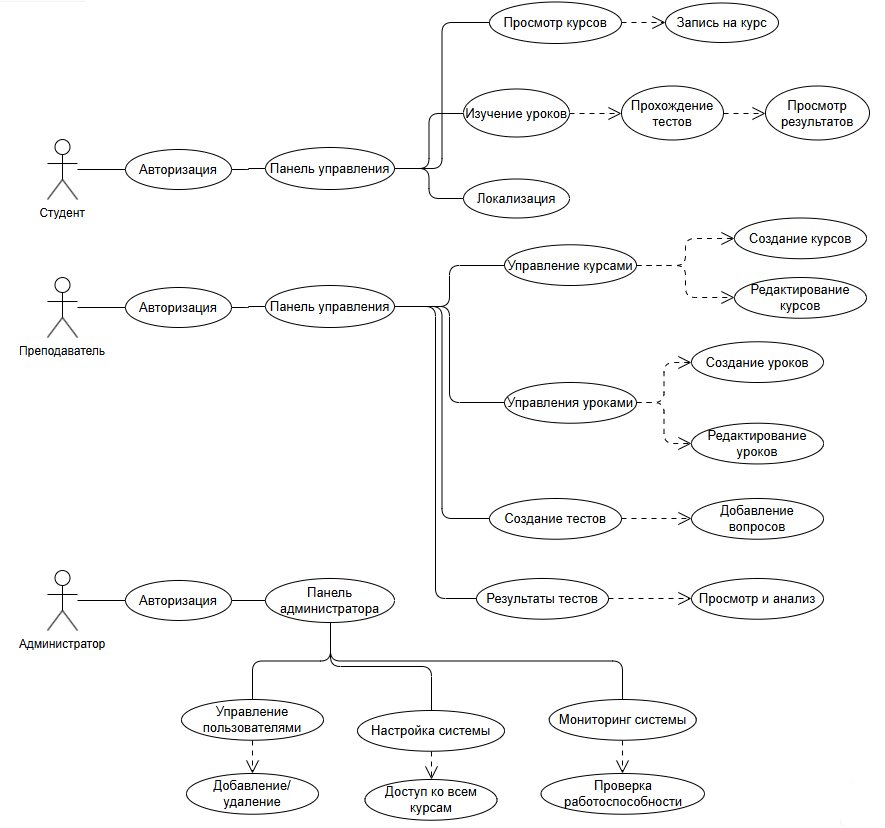
\includegraphics[width=1\linewidth]{UML}}
	\center{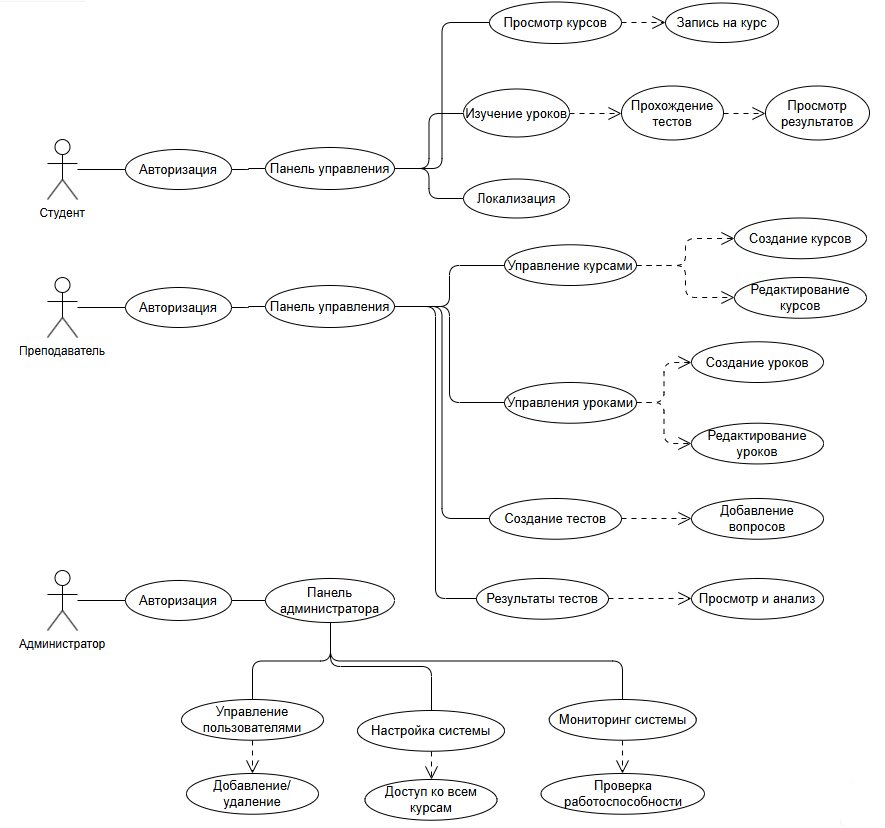
\includegraphics[width=1\linewidth]{UML}}
	\center{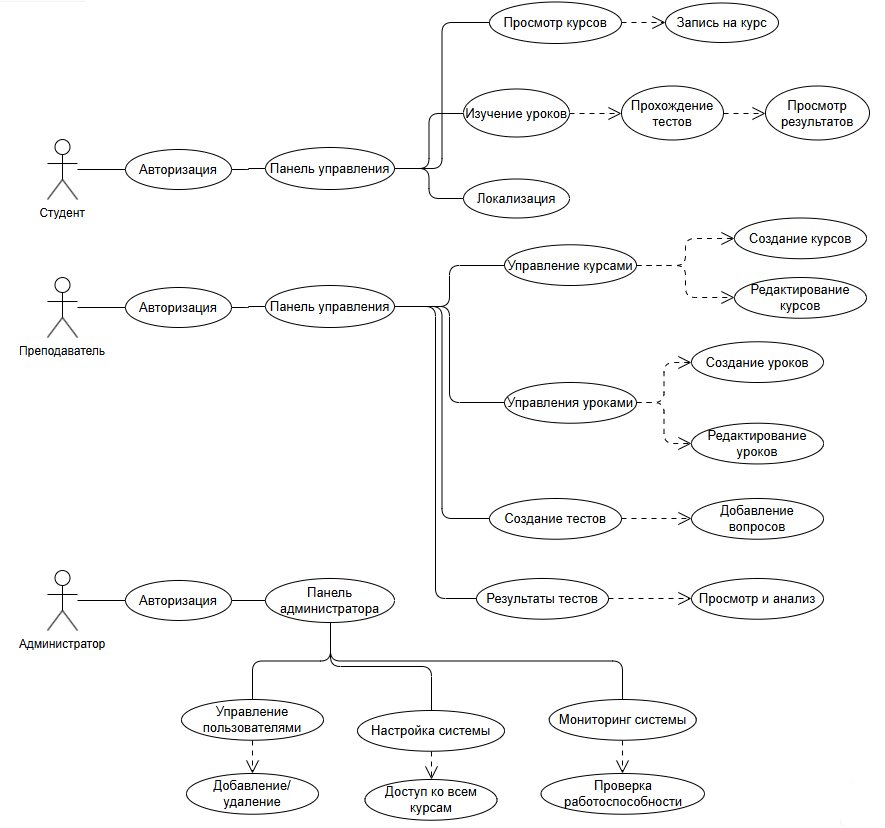
\includegraphics[width=1\linewidth]{UML}}
	\caption{Главная страница обучающей платформы}
	\label{main:image}
\end{figure}

На рисунке \ref{course:image} представлен интерфейс просмотра курса с динамическим отображением уроков и тестов по JavaScript.

\begin{figure}[ht]
	\center{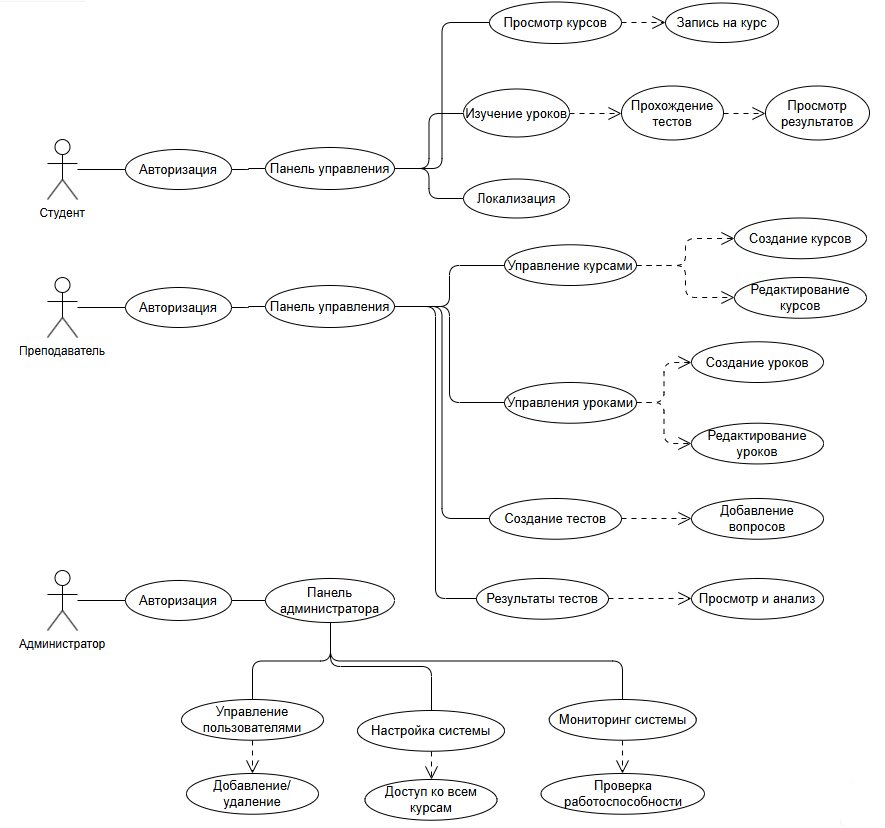
\includegraphics[width=1\linewidth]{UML}}
	\caption{Интерфейс просмотра курса}
	\label{course:image}
\end{figure}

На рисунке \ref{test:image} представлен интерфейс сдачи теста по JavaScript с динамической формой для выбора ответов.

\begin{figure}[ht]
	\center{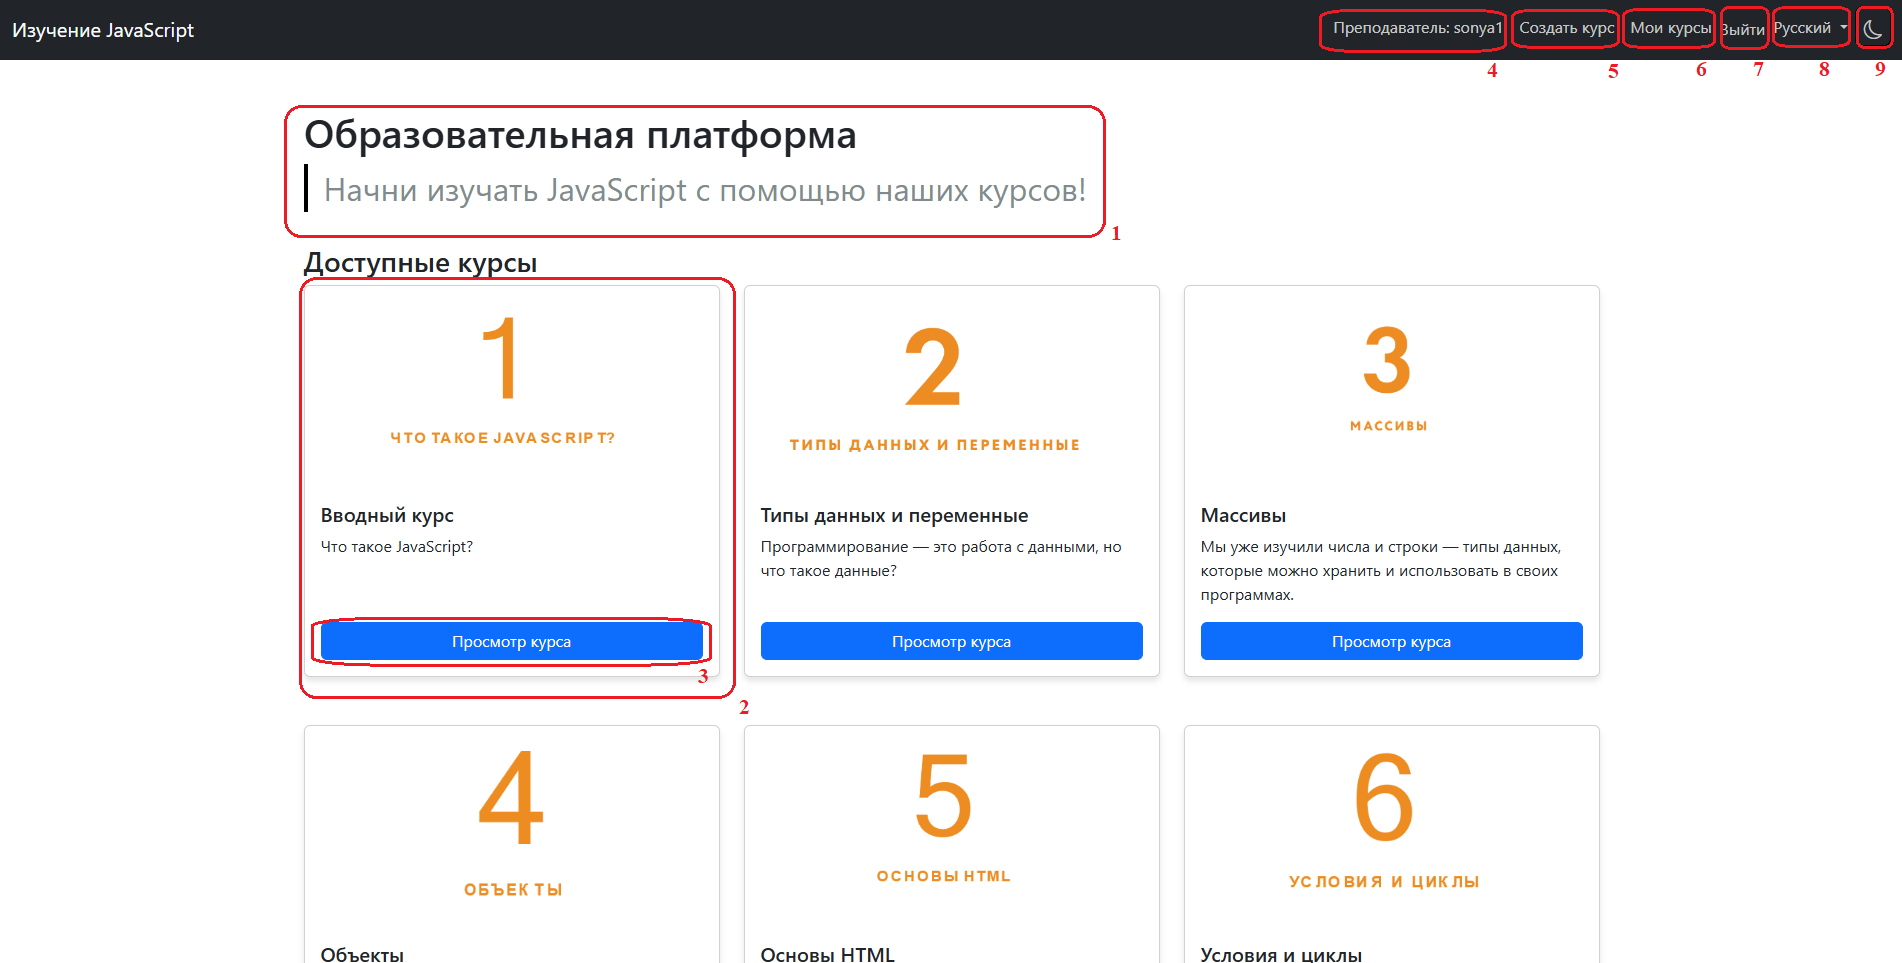
\includegraphics[width=1\linewidth]{курсы}}
	\caption{Интерфейс сдачи теста}
	\label{test:image}
\end{figure}